\begin{homework}
  \question Consider the adiabatic steam turbine shown below.
  \begin{center}
    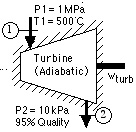
\includegraphics[width=0.3\textwidth]{steamTurb}
  \end{center}
  \begin{questionparts}
  \item Carefully plot the turbine process on the $h$-$s$ diagram and indicate the turbine work done on the plot.
  \item Using steam tables determine the specific work output of the turbine \answer{[1015 kJ/kg]}.
  \item Using steam tables determine the entropy generated by this process. \answer{[0.01 kJ/kg.K]}.
  \item Discuss these results and determine if this is a feasible turbine design.
  \end{questionparts}

  \question Adiabatic Evaluation of a R134a Compressor
  A young engineer was assigned to evaluate the compressor of a proposed R-134a refrigeration system shown below, and assumed it to be adiabatic.
  \begin{questionparts}
  \item Under this assumption, and ignoring kinetic and potential energy effects, determine the specific work input to the compressor \answer{[48.3 kJ/kg]}.
  \item His supervisor checked the results and told him that his assumption was incorrect and not physically feasible. On the $h$-$s$ diagram for R134a, draw the actual compression process (as assumed) as well as the equivalent isentropic compression process.
  \item Using the $h$-$s$ diagram, as well as relevant data evaluated at the inlet and outlet of the compressor, explain how she arrived at that conclusion.
  \end{questionparts}
  \newpage
  \question Previously, we provided a problem concerning a home refrigerator, and examining it's performance before and after adding an internal heat exchanger.
  \begin{center}
    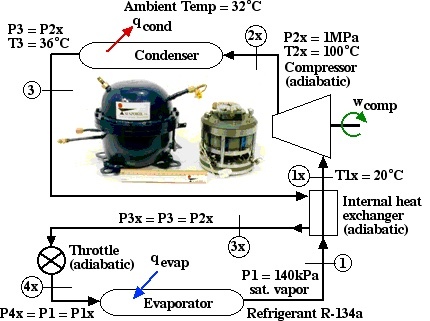
\includegraphics[width=0.5\textwidth]{ch4_HW_refrigHX}
  \end{center}
  \begin{questionparts}
  \item Plot the actual and the isentropic compressor processes on the enthalpy-entropy ($h$-$s$) diagram for both cases: with and without the internal heat exchanger.
  \item Using the R134a tables determine the actual compressor adiabatic efficiency ($\eta_C$) for both cases \answer{[75\%, 76\%]}
  \end{questionparts}

  \question A compressor is used to drive R134a through a heat pump.  R134a enters the compressor at a pressure $p_1$ = 400 kPa and a temperature $T_1$ = 40°C and leaves at a pressure $p_2$ = 1.6 MPa.  For the actual compressor, the exit tempearture is $T_2$ = 100°C.

  \begin{questionparts}
  \item Carefully plot the actual and isentropic compression processes on the $h$-$s$ diagram and indicate the actual and isentropic specific work done to drive the compressor on the plot.
  \item Using R134a refrigerant tables, determine the specific work required to drive the compressor \answer{[43.5 kJ/kg]}.
  \item Using R134a refrigerant tables, determine the adiabatic efficiency of the compressor \answer{[$\eta_C$ = 78\%]}.
  \item Discuss these results and determine if this is a feasible compressor design.
  \end{questionparts}
  \newpage
  \question In Example \ref{ex:T700} we did an ideal thermodynamic analysis of the General Electric T700 helicopter gas turbine engine, shown in the following schematic diagram:
  \begin{center}
    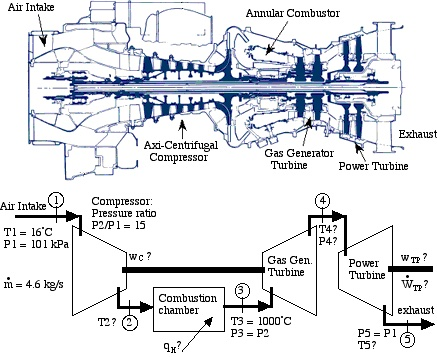
\includegraphics[width=.8\linewidth]{gas_turbine}
  \end{center}

  Notice again that there are two turbines operating on independent output shafts. The High Pressure (first) turbine, named the Gas Generator turbine, is directly connected by a shaft to the compressor. Its sole purpose is to drive the the compressor, thus the energy output of this turbine must equal the energy consumed by the compressor. The Low Pressure (second) turbine, named the Power turbine, is connected via gearing to the helicopter rotor.

  In Example \ref{ex:T700} we assumed that the compressor and both turbines were isentropic. In this exercise we wish to extend the analysis to non-isentropic compressor and turbines.

  Assume that the compressor adiabatic efficiency $\eta_C$ = 88\%, and that each turbine has an adiabatic efficiency $\eta_T$ = 86\%.

  \begin{questionparts}
  \item Sketch the entire process on an $h$-$s$ diagram, clearly showing the 5 stations on the diagram and the relevant isentropic and constant pressure lines. Indicate the relevant actual and isentropic work values on the sketch.
  \item Determine the actual energy consumed by the compressor \answer{[$w_{C,act}$ = 373 kJ/kg]}, and the actual temperature at the outlet of the compressor \answer{[$T_{2a}$ = 628K]}.
  \item Determine the heat energy absorbed by the working gas in the combustion chamber \answer{[$q_H$ = 709 kJ/kg]}.
  \item Determine the actual temperature [$T_{4a}$ = 934K] and the pressure [$P_4$ = 366 kPa] at the outlet of the gas generator turbine.
  \item Determine the actual temperature [$T_{5a}$] and energy output of the power turbine [$w_{PT,act}$ = 252 kJ/kg].
  \item Given that the mass flow rate of the working gas through the system is 4.6 kg/s, determine the actual power output of the power turbine \answer{[1161 kW]}.
  \item Determine the thermal efficiency ($\eta_{th}$) of the T700 gas turbine. Compare this value to the equivalent reversible thermal efficiency and discuss your results.
  \end{questionparts}

\end{homework}
